\documentclass[]{article}
\usepackage{lmodern}
\usepackage{amssymb,amsmath}
\usepackage{ifxetex,ifluatex}
\usepackage{fixltx2e} % provides \textsubscript
\ifnum 0\ifxetex 1\fi\ifluatex 1\fi=0 % if pdftex
  \usepackage[T1]{fontenc}
  \usepackage[utf8]{inputenc}
\else % if luatex or xelatex
  \ifxetex
    \usepackage{mathspec}
  \else
    \usepackage{fontspec}
  \fi
  \defaultfontfeatures{Ligatures=TeX,Scale=MatchLowercase}
\fi
% use upquote if available, for straight quotes in verbatim environments
\IfFileExists{upquote.sty}{\usepackage{upquote}}{}
% use microtype if available
\IfFileExists{microtype.sty}{%
\usepackage{microtype}
\UseMicrotypeSet[protrusion]{basicmath} % disable protrusion for tt fonts
}{}
\usepackage[margin=1in]{geometry}
\usepackage{hyperref}
\hypersetup{unicode=true,
            pdfauthor={Salvatore A. Sidoti \textbar{} PhD Candidate \textbar{} Behavioral Ecology \textbar{} The Department of Evolution, Ecology \& Organismal Biology \textbar{} sidoti.23@osu.edu},
            pdfborder={0 0 0},
            breaklinks=true}
\urlstyle{same}  % don't use monospace font for urls
\usepackage{color}
\usepackage{fancyvrb}
\newcommand{\VerbBar}{|}
\newcommand{\VERB}{\Verb[commandchars=\\\{\}]}
\DefineVerbatimEnvironment{Highlighting}{Verbatim}{commandchars=\\\{\}}
% Add ',fontsize=\small' for more characters per line
\usepackage{framed}
\definecolor{shadecolor}{RGB}{248,248,248}
\newenvironment{Shaded}{\begin{snugshade}}{\end{snugshade}}
\newcommand{\AlertTok}[1]{\textcolor[rgb]{0.94,0.16,0.16}{#1}}
\newcommand{\AnnotationTok}[1]{\textcolor[rgb]{0.56,0.35,0.01}{\textbf{\textit{#1}}}}
\newcommand{\AttributeTok}[1]{\textcolor[rgb]{0.77,0.63,0.00}{#1}}
\newcommand{\BaseNTok}[1]{\textcolor[rgb]{0.00,0.00,0.81}{#1}}
\newcommand{\BuiltInTok}[1]{#1}
\newcommand{\CharTok}[1]{\textcolor[rgb]{0.31,0.60,0.02}{#1}}
\newcommand{\CommentTok}[1]{\textcolor[rgb]{0.56,0.35,0.01}{\textit{#1}}}
\newcommand{\CommentVarTok}[1]{\textcolor[rgb]{0.56,0.35,0.01}{\textbf{\textit{#1}}}}
\newcommand{\ConstantTok}[1]{\textcolor[rgb]{0.00,0.00,0.00}{#1}}
\newcommand{\ControlFlowTok}[1]{\textcolor[rgb]{0.13,0.29,0.53}{\textbf{#1}}}
\newcommand{\DataTypeTok}[1]{\textcolor[rgb]{0.13,0.29,0.53}{#1}}
\newcommand{\DecValTok}[1]{\textcolor[rgb]{0.00,0.00,0.81}{#1}}
\newcommand{\DocumentationTok}[1]{\textcolor[rgb]{0.56,0.35,0.01}{\textbf{\textit{#1}}}}
\newcommand{\ErrorTok}[1]{\textcolor[rgb]{0.64,0.00,0.00}{\textbf{#1}}}
\newcommand{\ExtensionTok}[1]{#1}
\newcommand{\FloatTok}[1]{\textcolor[rgb]{0.00,0.00,0.81}{#1}}
\newcommand{\FunctionTok}[1]{\textcolor[rgb]{0.00,0.00,0.00}{#1}}
\newcommand{\ImportTok}[1]{#1}
\newcommand{\InformationTok}[1]{\textcolor[rgb]{0.56,0.35,0.01}{\textbf{\textit{#1}}}}
\newcommand{\KeywordTok}[1]{\textcolor[rgb]{0.13,0.29,0.53}{\textbf{#1}}}
\newcommand{\NormalTok}[1]{#1}
\newcommand{\OperatorTok}[1]{\textcolor[rgb]{0.81,0.36,0.00}{\textbf{#1}}}
\newcommand{\OtherTok}[1]{\textcolor[rgb]{0.56,0.35,0.01}{#1}}
\newcommand{\PreprocessorTok}[1]{\textcolor[rgb]{0.56,0.35,0.01}{\textit{#1}}}
\newcommand{\RegionMarkerTok}[1]{#1}
\newcommand{\SpecialCharTok}[1]{\textcolor[rgb]{0.00,0.00,0.00}{#1}}
\newcommand{\SpecialStringTok}[1]{\textcolor[rgb]{0.31,0.60,0.02}{#1}}
\newcommand{\StringTok}[1]{\textcolor[rgb]{0.31,0.60,0.02}{#1}}
\newcommand{\VariableTok}[1]{\textcolor[rgb]{0.00,0.00,0.00}{#1}}
\newcommand{\VerbatimStringTok}[1]{\textcolor[rgb]{0.31,0.60,0.02}{#1}}
\newcommand{\WarningTok}[1]{\textcolor[rgb]{0.56,0.35,0.01}{\textbf{\textit{#1}}}}
\usepackage{graphicx,grffile}
\makeatletter
\def\maxwidth{\ifdim\Gin@nat@width>\linewidth\linewidth\else\Gin@nat@width\fi}
\def\maxheight{\ifdim\Gin@nat@height>\textheight\textheight\else\Gin@nat@height\fi}
\makeatother
% Scale images if necessary, so that they will not overflow the page
% margins by default, and it is still possible to overwrite the defaults
% using explicit options in \includegraphics[width, height, ...]{}
\setkeys{Gin}{width=\maxwidth,height=\maxheight,keepaspectratio}
\IfFileExists{parskip.sty}{%
\usepackage{parskip}
}{% else
\setlength{\parindent}{0pt}
\setlength{\parskip}{6pt plus 2pt minus 1pt}
}
\setlength{\emergencystretch}{3em}  % prevent overfull lines
\providecommand{\tightlist}{%
  \setlength{\itemsep}{0pt}\setlength{\parskip}{0pt}}
\setcounter{secnumdepth}{0}
% Redefines (sub)paragraphs to behave more like sections
\ifx\paragraph\undefined\else
\let\oldparagraph\paragraph
\renewcommand{\paragraph}[1]{\oldparagraph{#1}\mbox{}}
\fi
\ifx\subparagraph\undefined\else
\let\oldsubparagraph\subparagraph
\renewcommand{\subparagraph}[1]{\oldsubparagraph{#1}\mbox{}}
\fi

%%% Use protect on footnotes to avoid problems with footnotes in titles
\let\rmarkdownfootnote\footnote%
\def\footnote{\protect\rmarkdownfootnote}

%%% Change title format to be more compact
\usepackage{titling}

% Create subtitle command for use in maketitle
\newcommand{\subtitle}[1]{
  \posttitle{
    \begin{center}\large#1\end{center}
    }
}

\setlength{\droptitle}{-2em}

  \title{An Introduction with Examples in R\\
Principal Component Analysis:}
    \pretitle{\vspace{\droptitle}\centering\huge}
  \posttitle{\par}
    \author{Salvatore A. Sidoti \textbar{} PhD Candidate \textbar{} Behavioral
Ecology \textbar{} The Department of Evolution, Ecology \& Organismal
Biology \textbar{}
\href{mailto:sidoti.23@osu.edu}{\nolinkurl{sidoti.23@osu.edu}}}
    \preauthor{\centering\large\emph}
  \postauthor{\par}
      \predate{\centering\large\emph}
  \postdate{\par}
    \date{2019-02-12}

\usepackage{booktabs}
\usepackage{longtable}
\usepackage{array}
\usepackage{multirow}
\usepackage{wrapfig}
\usepackage{float}
\usepackage{colortbl}
\usepackage{pdflscape}
\usepackage{tabu}
\usepackage{threeparttable}
\usepackage{threeparttablex}
\usepackage[normalem]{ulem}
\usepackage{makecell}
\usepackage{xcolor}

\begin{document}
\maketitle

\hypertarget{introduction}{%
\section{Introduction}\label{introduction}}

Principle component analysis (PCA) distributes the variation in a
multivariate dataset across \emph{components}. The PCA allows us to
visualize patterns that would not be apparent with common graphical
techniques. Linear algebra is at the heart of the PCA, but this
discussion will be light on mathematical theory. Instead, you can expect
a gentle introduction to the topic, which will include how this
ordination technique is carried out in R.

\hypertarget{accomplishing-the-pca-manually}{%
\section{\texorpdfstring{Accomplishing the PCA
\emph{Manually}}{Accomplishing the PCA Manually}}\label{accomplishing-the-pca-manually}}

With the powerful tools available to us in R, there is no need to
conduct a PCA manually. Contained within one line of code, R has native
functions which can handle the heavy-lifting for us. My goal for the
\emph{manual} PCA is to expose you to the terminology and concepts in
PCA. As such, you will be better prepared to defend your analysis.

\hypertarget{motivating-example---wolf-spider-morphometrics}{%
\subsection{Motivating example - wolf spider
morphometrics}\label{motivating-example---wolf-spider-morphometrics}}

The original motivation for this analysis was to establish a standard
algorithm to determine the ``size'' of a wolf spider. One way to
accomplish this is with a PCA of morphometric characteristics. The
parameters which possess the highest degree of variation will be the
most optimal predictor of animal size.

\begin{center}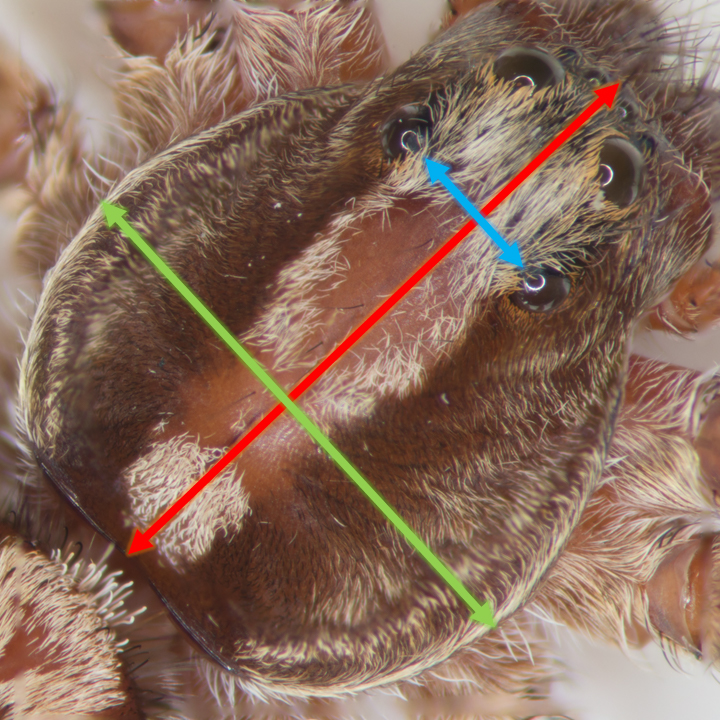
\includegraphics[width=10in]{morpho} \end{center}

\emph{Blue: interocular distance, Green: carapace width, Red: carapace
length}

Descriptive Statistics

\begin{Shaded}
\begin{Highlighting}[]
\CommentTok{# Load the full data set}
\KeywordTok{load}\NormalTok{(}\StringTok{"morpho_complete.Rdata"}\NormalTok{)}

\CommentTok{# Eliminate factor variables & untransformed weights from full dataset}
\NormalTok{morpho <-}\StringTok{ }\NormalTok{morpho_complete[,}\OperatorTok{-}\KeywordTok{c}\NormalTok{(}\DecValTok{1}\NormalTok{,}\DecValTok{2}\NormalTok{,}\DecValTok{6}\NormalTok{)]}

\NormalTok{morpho.stats <-}\StringTok{ }\KeywordTok{round}\NormalTok{(}\KeywordTok{stat.desc}\NormalTok{(morpho, }\DataTypeTok{basic =} \OtherTok{FALSE}\NormalTok{), }\DataTypeTok{digits =} \DecValTok{3}\NormalTok{)}
\KeywordTok{kable}\NormalTok{(morpho.stats, }\DataTypeTok{caption =} \StringTok{"Descriptive Statistics"}\NormalTok{) }\OperatorTok
\StringTok{  }\KeywordTok{kable_styling}\NormalTok{(}\DataTypeTok{bootstrap_options =} \KeywordTok{c}\NormalTok{(}\StringTok{"striped"}\NormalTok{, }\StringTok{"hover"}\NormalTok{, }\StringTok{"condensed"}\NormalTok{, }\StringTok{"responsive"}\NormalTok{), }\DataTypeTok{full_width =}\NormalTok{ F)}
\end{Highlighting}
\end{Shaded}

\begin{table}[t]

\caption{\label{tab:unnamed-chunk-3}Descriptive Statistics}
\centering
\begin{tabular}{l|r|r|r|r}
\hline
  & interoc & cwidth & clength & T.weight\\
\hline
median & 0.798 & 2.975 & 3.706 & 1.740\\
\hline
mean & 0.799 & 2.991 & 3.691 & 1.742\\
\hline
SE.mean & 0.005 & 0.020 & 0.020 & 0.004\\
\hline
CI.mean.0.95 & 0.011 & 0.039 & 0.039 & 0.008\\
\hline
var & 0.002 & 0.028 & 0.028 & 0.001\\
\hline
std.dev & 0.046 & 0.166 & 0.167 & 0.033\\
\hline
coef.var & 0.058 & 0.055 & 0.045 & 0.019\\
\hline
\end{tabular}
\end{table}

\begin{Shaded}
\begin{Highlighting}[]
\KeywordTok{pairs.panels}\NormalTok{(}
\NormalTok{  morpho,}
  \DataTypeTok{main =} \StringTok{"Wolf Spider Morphometrics - Correlation Summary"}\NormalTok{,}
  \DataTypeTok{gap =} \DecValTok{0}\NormalTok{, }\CommentTok{# set to zero for no gap between plot panels}
  \DataTypeTok{lm =} \OtherTok{TRUE}\NormalTok{, }\CommentTok{# draw linear regression lines for pairs}
  \DataTypeTok{stars =} \OtherTok{TRUE}\NormalTok{, }\CommentTok{# display significance}
  \DataTypeTok{bg =} \KeywordTok{c}\NormalTok{(}\StringTok{"red"}\NormalTok{, }\StringTok{"blue"}\NormalTok{)[morpho_complete}\OperatorTok{$}\NormalTok{sex], }\CommentTok{# color based on sex }
  \DataTypeTok{pch =} \DecValTok{21}\NormalTok{) }\CommentTok{# data point shape}
\end{Highlighting}
\end{Shaded}

\begin{center}\includegraphics{morpho-pca_files/figure-latex/unnamed-chunk-4-1} \end{center}

\hypertarget{covariance-or-correlation}{%
\subsection{Covariance or
Correlation?}\label{covariance-or-correlation}}

PCA is a dimensionality reduction technique that allows us to see latent
patterns in the data. To do this, the PCA is based heavily on concepts
in linear algebra: eigenvalues and eigenvectors are at the heart of the
PCA. First, we need to establish whether the metrics in our dataset are
\emph{like} or \emph{mixed}. If the dataset contains the same units of
measure across all of the variables -- i.e.~all variables are weights in
grams -- we \emph{standardize} the data via mean-centering and employ a
\emph{covariance} matrix. However, if our data contains mixed units --
like the morphometric data in this example -- we mean-center the data,
divide by the standard deviation, and employ a \emph{correlation}
matrix. Which matrix you choose becomes essential when setting the
parameters of the built-in PCA functions in R.

Our data has \emph{mixed} metrics - weight (mg) and linear measures
(mm).

\hypertarget{standardize-the-data-mean-center-and-divide-by-the-standard-deviation}{%
\subsection{Standardize the Data: Mean-center and Divide by the Standard
Deviation}\label{standardize-the-data-mean-center-and-divide-by-the-standard-deviation}}

\begin{Shaded}
\begin{Highlighting}[]
\NormalTok{standardize <-}\StringTok{ }\ControlFlowTok{function}\NormalTok{(x) \{(x }\OperatorTok{-}\StringTok{ }\KeywordTok{mean}\NormalTok{(x))}\OperatorTok{/}\KeywordTok{sd}\NormalTok{(x)\}}

\CommentTok{# Eliminate factor variables & untransformed weights from the scaled data}
\NormalTok{my.scaled.data <-}\StringTok{ }\KeywordTok{as.data.frame}\NormalTok{(}\KeywordTok{apply}\NormalTok{(morpho, }\DecValTok{2}\NormalTok{, standardize))}

\KeywordTok{ggplot}\NormalTok{(my.scaled.data, }\KeywordTok{aes}\NormalTok{(interoc, cwidth)) }\OperatorTok{+}
\StringTok{  }\KeywordTok{geom_point}\NormalTok{(}\DataTypeTok{size =} \DecValTok{2}\NormalTok{) }\OperatorTok{+}
\StringTok{  }\KeywordTok{geom_smooth}\NormalTok{(}\DataTypeTok{method =} \StringTok{'lm'}\NormalTok{) }\OperatorTok{+}
\StringTok{  }\KeywordTok{ggtitle}\NormalTok{(}\StringTok{"Plot of Interoccular Distance and Carapace Width"}\NormalTok{) }\OperatorTok{+}
\StringTok{  }\KeywordTok{theme}\NormalTok{(}\DataTypeTok{plot.title =} \KeywordTok{element_text}\NormalTok{(}\DataTypeTok{hjust =} \FloatTok{0.5}\NormalTok{)) }\CommentTok{# center plot title}
\end{Highlighting}
\end{Shaded}

\begin{center}\includegraphics{morpho-pca_files/figure-latex/fig1-1} \end{center}

\hypertarget{find-the-eigenvalues-eigenvectors}{%
\subsection{Find the Eigenvalues \&
Eigenvectors}\label{find-the-eigenvalues-eigenvectors}}

\begin{Shaded}
\begin{Highlighting}[]
\CommentTok{# Calculate correlation matrix}
\NormalTok{my.cor <-}\StringTok{ }\KeywordTok{cor}\NormalTok{(my.scaled.data)}

\CommentTok{# Save the eigenvalues of the correllation matrix}
\NormalTok{my.eigen <-}\StringTok{ }\KeywordTok{eigen}\NormalTok{(my.cor)}

\CommentTok{# Rename matrix rows and columns for easier interpretation}
\KeywordTok{rownames}\NormalTok{(my.eigen}\OperatorTok{$}\NormalTok{vectors) <-}\StringTok{ }\KeywordTok{c}\NormalTok{(}\StringTok{"interoc"}\NormalTok{, }\StringTok{"cwidth"}\NormalTok{, }\StringTok{"clength"}\NormalTok{, }\StringTok{"T.weight"}\NormalTok{)}
\KeywordTok{colnames}\NormalTok{(my.eigen}\OperatorTok{$}\NormalTok{vectors) <-}\StringTok{ }\KeywordTok{c}\NormalTok{(}\StringTok{"PC1"}\NormalTok{, }\StringTok{"PC2"}\NormalTok{, }\StringTok{"PC3"}\NormalTok{, }\StringTok{"PC4"}\NormalTok{)}
\end{Highlighting}
\end{Shaded}

\begin{wraptable}{l}{0pt}[t]

\caption{\label{tab:unnamed-chunk-6}Eigenvectors}
\centering
\begin{tabular}{>{\bfseries}l|r|r|r|r}
\hline
  & PC1 & PC2 & PC3 & PC4\\
\hline
interoc & -0.4972563 & -0.2503917 & 0.8251161 & -0.0960398\\
\hline
cwidth & -0.5318709 & -0.3465188 & -0.4947682 & -0.5935002\\
\hline
clength & -0.5759897 & -0.0463106 & -0.2715924 & 0.7696290\\
\hline
T.weight & -0.3715984 & 0.9028201 & 0.0250084 & -0.2149537\\
\hline
\end{tabular}
\end{wraptable}

\begin{table}[t]

\caption{\label{tab:unnamed-chunk-7}Eigenvalues For PCs}
\centering
\begin{tabular}{>{\bfseries}l|r}
\hline
PC & eigenvalues\\
\hline
PC1 & 2.7104296\\
\hline
PC2 & 0.7607956\\
\hline
PC3 & 0.4127988\\
\hline
PC4 & 0.1159759\\
\hline
\end{tabular}
\end{table}

Each column in the table above (left) is an eigenvector. Each
eigenvector is a \emph{principal component} (PC) with its eigenvalue.
These eigenvalues are given in the right table above. The eigenvalues
are used to identify which principal component(s) have the strongest
correlation with the overall dataset: the higher the eigenvalue, the
stronger its correlation. Each eigenvector is a \emph{normalized linear
combination} of the variables \texttt{interoc}, \texttt{cwidth},
\texttt{clength}, \texttt{T.weight}.

The coefficients are known as \emph{loadings} which are values
\(\small[-1, 1]\). We can see that the variables of interest in PC1
trend together due to all of the coefficients having the same sign.

Note that the sum of the eigenvalues equals the total variance of the
scaled data

\begin{Shaded}
\begin{Highlighting}[]
\KeywordTok{sum}\NormalTok{(my.eigen}\OperatorTok{$}\NormalTok{values)}
\end{Highlighting}
\end{Shaded}

\begin{verbatim}
## [1] 4
\end{verbatim}

\begin{Shaded}
\begin{Highlighting}[]
\KeywordTok{sum}\NormalTok{(}
  \KeywordTok{var}\NormalTok{(my.scaled.data[,}\DecValTok{1}\NormalTok{]),}
  \KeywordTok{var}\NormalTok{(my.scaled.data[,}\DecValTok{2}\NormalTok{]),}
  \KeywordTok{var}\NormalTok{(my.scaled.data[,}\DecValTok{3}\NormalTok{]),}
  \KeywordTok{var}\NormalTok{(my.scaled.data[,}\DecValTok{4}\NormalTok{]))}
\end{Highlighting}
\end{Shaded}

\begin{verbatim}
## [1] 4
\end{verbatim}

\hypertarget{amount-of-variation-captured-by-the-pcs-in-the-dataset}{%
\subsection{Amount of Variation Captured by the PCs in the
Dataset}\label{amount-of-variation-captured-by-the-pcs-in-the-dataset}}

Take each eigenvalue and divide it by the total of all eigenvalues --
the total variation in the dataset -- then multiply by 100. This
calculation yields a table with the percent variation for each PC.

\begin{Shaded}
\begin{Highlighting}[]
\NormalTok{pc1.var <-}\StringTok{ }\DecValTok{100}\OperatorTok{*}\KeywordTok{round}\NormalTok{(my.eigen}\OperatorTok{$}\NormalTok{values[}\DecValTok{1}\NormalTok{]}\OperatorTok{/}\KeywordTok{sum}\NormalTok{(my.eigen}\OperatorTok{$}\NormalTok{values), }\DataTypeTok{digits =} \DecValTok{3}\NormalTok{)}
\NormalTok{pc2.var <-}\StringTok{ }\DecValTok{100}\OperatorTok{*}\KeywordTok{round}\NormalTok{(my.eigen}\OperatorTok{$}\NormalTok{values[}\DecValTok{2}\NormalTok{]}\OperatorTok{/}\KeywordTok{sum}\NormalTok{(my.eigen}\OperatorTok{$}\NormalTok{values), }\DataTypeTok{digits =} \DecValTok{3}\NormalTok{)}
\NormalTok{pc3.var <-}\StringTok{ }\DecValTok{100}\OperatorTok{*}\KeywordTok{round}\NormalTok{(my.eigen}\OperatorTok{$}\NormalTok{values[}\DecValTok{3}\NormalTok{]}\OperatorTok{/}\KeywordTok{sum}\NormalTok{(my.eigen}\OperatorTok{$}\NormalTok{values), }\DataTypeTok{digits =} \DecValTok{3}\NormalTok{)}
\NormalTok{pc4.var <-}\StringTok{ }\DecValTok{100}\OperatorTok{*}\KeywordTok{round}\NormalTok{(my.eigen}\OperatorTok{$}\NormalTok{values[}\DecValTok{4}\NormalTok{]}\OperatorTok{/}\KeywordTok{sum}\NormalTok{(my.eigen}\OperatorTok{$}\NormalTok{values), }\DataTypeTok{digits =} \DecValTok{3}\NormalTok{)}

\NormalTok{pc <-}\StringTok{ }\KeywordTok{data.frame}\NormalTok{(}\DataTypeTok{PC =} \KeywordTok{c}\NormalTok{(}\StringTok{"PC1"}\NormalTok{, }\StringTok{"PC2"}\NormalTok{, }\StringTok{"PC3"}\NormalTok{, }\StringTok{"PC4"}\NormalTok{),}
                 \DataTypeTok{Percentage =} \KeywordTok{c}\NormalTok{(pc1.var, pc2.var, pc3.var, pc4.var))}

\KeywordTok{kable}\NormalTok{(pc, }\DataTypeTok{caption =} \StringTok{"Amount of Variation Captured by PCs"}\NormalTok{) }\OperatorTok
\StringTok{  }\KeywordTok{kable_styling}\NormalTok{(}\DataTypeTok{bootstrap_options =} \KeywordTok{c}\NormalTok{(}\StringTok{"striped"}\NormalTok{, }\StringTok{"hover"}\NormalTok{, }\StringTok{"condensed"}\NormalTok{, }\StringTok{"responsive"}\NormalTok{), }\DataTypeTok{full_width =}\NormalTok{ F)}
\end{Highlighting}
\end{Shaded}

\begin{table}[t]

\caption{\label{tab:unnamed-chunk-9}Amount of Variation Captured by PCs}
\centering
\begin{tabular}{l|r}
\hline
PC & Percentage\\
\hline
PC1 & 67.8\\
\hline
PC2 & 19.0\\
\hline
PC3 & 10.3\\
\hline
PC4 & 2.9\\
\hline
\end{tabular}
\end{table}

The total variation should sum to \textasciitilde{}100\% depending on
rounding error:

\begin{Shaded}
\begin{Highlighting}[]
\KeywordTok{sum}\NormalTok{(pc1.var, pc2.var, pc3.var, pc4.var)}
\end{Highlighting}
\end{Shaded}

\begin{verbatim}
## [1] 100
\end{verbatim}

\hypertarget{what-are-the-pca-scores}{%
\subsection{What are the PCA
``scores''?}\label{what-are-the-pca-scores}}

Express the loadings and scaled data as matrices, then multiply them
together. The result is a new matrix which expresses the data in terms
of the PCs. These are the PCA \emph{scores}.

\begin{Shaded}
\begin{Highlighting}[]
\NormalTok{loadings <-}\StringTok{ }\NormalTok{my.eigen}\OperatorTok{$}\NormalTok{vectors}
\NormalTok{my.scaled.matrix <-}\StringTok{ }\KeywordTok{as.matrix}\NormalTok{(my.scaled.data)}
\CommentTok{# the function %*% is matrix multiplication}
\NormalTok{scores <-}\StringTok{ }\NormalTok{my.scaled.matrix }\OperatorTok\StringTok{ }\NormalTok{loadings}
\NormalTok{sd <-}\StringTok{ }\KeywordTok{sqrt}\NormalTok{(my.eigen}\OperatorTok{$}\NormalTok{values)}
\KeywordTok{rownames}\NormalTok{(loadings) <-}\StringTok{ }\KeywordTok{colnames}\NormalTok{(my.scaled.data)}

\KeywordTok{kable}\NormalTok{(}\KeywordTok{head}\NormalTok{(scores), }\DataTypeTok{caption =} \StringTok{"PCA Scores - First Six Rows"}\NormalTok{) }\OperatorTok
\StringTok{  }\KeywordTok{kable_styling}\NormalTok{(}\DataTypeTok{bootstrap_options =} \KeywordTok{c}\NormalTok{(}\StringTok{"striped"}\NormalTok{, }\StringTok{"hover"}\NormalTok{, }\StringTok{"condensed"}\NormalTok{, }\StringTok{"responsive"}\NormalTok{),}
                \DataTypeTok{full_width =}\NormalTok{ F)}
\end{Highlighting}
\end{Shaded}

\begin{table}[t]

\caption{\label{tab:unnamed-chunk-11}PCA Scores - First Six Rows}
\centering
\begin{tabular}{r|r|r|r}
\hline
PC1 & PC2 & PC3 & PC4\\
\hline
-2.2600333 & 0.4795785 & 0.1963305 & -0.0511398\\
\hline
-1.2140895 & 1.0327956 & 0.0184971 & 0.0859329\\
\hline
-2.9229522 & 0.7366524 & -0.3902236 & 0.5873086\\
\hline
-1.0989536 & 1.0164286 & 0.0283129 & 0.0653717\\
\hline
-0.5060125 & 1.8150422 & 0.8229882 & 0.6191984\\
\hline
-0.3073533 & 0.8777547 & 0.0583005 & -0.0498082\\
\hline
\end{tabular}
\end{table}

\hypertarget{accomplishing-the-pca-with-native-r-functions}{%
\section{Accomplishing the PCA with Native R
Functions}\label{accomplishing-the-pca-with-native-r-functions}}

The function \texttt{prcomp} is the primary tool for PCA in base R.

\begin{Shaded}
\begin{Highlighting}[]
\NormalTok{pca_morpho <-}\StringTok{ }\KeywordTok{prcomp}\NormalTok{(morpho, }\DataTypeTok{center =} \OtherTok{TRUE}\NormalTok{, }\DataTypeTok{scale. =} \OtherTok{TRUE}\NormalTok{)}

\CommentTok{# Show the variables in the class "prcomp"}
\KeywordTok{ls}\NormalTok{(pca_morpho)}
\end{Highlighting}
\end{Shaded}

\begin{verbatim}
## [1] "center"   "rotation" "scale"    "sdev"     "x"
\end{verbatim}

Rotations are often referred to as the ``loadings'' of a PCA.

\begin{Shaded}
\begin{Highlighting}[]
\NormalTok{pca_loadings <-}\StringTok{ }\NormalTok{pca_morpho}\OperatorTok{$}\NormalTok{rotation}
\KeywordTok{kable}\NormalTok{(pca_loadings, }\DataTypeTok{caption =} \StringTok{"PCA Loadings"}\NormalTok{) }\OperatorTok
\StringTok{  }\KeywordTok{kable_styling}\NormalTok{(}\DataTypeTok{bootstrap_options =} \KeywordTok{c}\NormalTok{(}\StringTok{"striped"}\NormalTok{, }\StringTok{"hover"}\NormalTok{, }\StringTok{"condensed"}\NormalTok{, }\StringTok{"responsive"}\NormalTok{),}
                \DataTypeTok{full_width =}\NormalTok{ F)}
\end{Highlighting}
\end{Shaded}

\begin{table}[t]

\caption{\label{tab:unnamed-chunk-13}PCA Loadings}
\centering
\begin{tabular}{l|r|r|r|r}
\hline
  & PC1 & PC2 & PC3 & PC4\\
\hline
interoc & -0.4972563 & -0.2503917 & 0.8251161 & -0.0960398\\
\hline
cwidth & -0.5318709 & -0.3465188 & -0.4947682 & -0.5935002\\
\hline
clength & -0.5759897 & -0.0463106 & -0.2715924 & 0.7696290\\
\hline
T.weight & -0.3715984 & 0.9028201 & 0.0250084 & -0.2149537\\
\hline
\end{tabular}
\end{table}

Summary output of the PCA:

\begin{Shaded}
\begin{Highlighting}[]
\NormalTok{pca_summary <-}\StringTok{ }\KeywordTok{summary}\NormalTok{(pca_morpho)}\OperatorTok{$}\NormalTok{importance }\OperatorTok
\StringTok{  }\KeywordTok{as.data.frame}\NormalTok{()}
\KeywordTok{kable}\NormalTok{(pca_summary, }\DataTypeTok{caption =} \StringTok{"PCA Summary"}\NormalTok{) }\OperatorTok
\StringTok{  }\KeywordTok{kable_styling}\NormalTok{(}\DataTypeTok{bootstrap_options =} \KeywordTok{c}\NormalTok{(}\StringTok{"striped"}\NormalTok{, }\StringTok{"hover"}\NormalTok{, }\StringTok{"condensed"}\NormalTok{, }\StringTok{"responsive"}\NormalTok{), }\DataTypeTok{full_width =}\NormalTok{ F)}
\end{Highlighting}
\end{Shaded}

\begin{table}[t]

\caption{\label{tab:unnamed-chunk-14}PCA Summary}
\centering
\begin{tabular}{l|r|r|r|r}
\hline
  & PC1 & PC2 & PC3 & PC4\\
\hline
Standard deviation & 1.646338 & 0.872236 & 0.6424942 & 0.3405524\\
\hline
Proportion of Variance & 0.677610 & 0.190200 & 0.1032000 & 0.0289900\\
\hline
Cumulative Proportion & 0.677610 & 0.867810 & 0.9710100 & 1.0000000\\
\hline
\end{tabular}
\end{table}

\hypertarget{orthogonality-of-pcs}{%
\subsection{Orthogonality of PCs}\label{orthogonality-of-pcs}}

\begin{Shaded}
\begin{Highlighting}[]
\KeywordTok{pairs.panels}\NormalTok{(}
\NormalTok{  pca_morpho}\OperatorTok{$}\NormalTok{x,}
  \DataTypeTok{main =} \StringTok{"PCA Correlation Summary"}\NormalTok{,}
  \DataTypeTok{gap =} \DecValTok{0}\NormalTok{, }\CommentTok{# set to zero for no gap between plot panels}
  \DataTypeTok{lm =} \OtherTok{TRUE}\NormalTok{, }\CommentTok{# draw linear regression lines for pairs}
  \DataTypeTok{stars =} \OtherTok{TRUE}\NormalTok{, }\CommentTok{# display significance}
  \DataTypeTok{bg =} \KeywordTok{c}\NormalTok{(}\StringTok{"red"}\NormalTok{, }\StringTok{"blue"}\NormalTok{)[morpho_complete}\OperatorTok{$}\NormalTok{sex], }\CommentTok{# color based on sex }
  \DataTypeTok{pch =} \DecValTok{21}\NormalTok{) }\CommentTok{# data point shape}
\end{Highlighting}
\end{Shaded}

\begin{center}\includegraphics{morpho-pca_files/figure-latex/unnamed-chunk-15-1} \end{center}

PCs are \emph{orthogonal vectors}. Thus, the correlation coefficients
equal zero for all possible pairwise combinations of PCs. Therefore, it
is often used as a precursor to predictive modeling procedures as
multicollinearity is eliminated.

\hypertarget{biplot}{%
\subsection{Biplot}\label{biplot}}

The \emph{biplot} is the primary visualization tool for PCA.

\begin{Shaded}
\begin{Highlighting}[]
\CommentTok{# Plot without ID labels}
\NormalTok{g <-}\StringTok{ }\KeywordTok{ggbiplot}\NormalTok{(pca_morpho,}
              \DataTypeTok{obs.scale =} \DecValTok{1}\NormalTok{,}
              \DataTypeTok{var.scale =} \DecValTok{1}\NormalTok{,}
              \DataTypeTok{groups =}\NormalTok{ morpho_complete}\OperatorTok{$}\NormalTok{sex,}
              \DataTypeTok{ellipse =} \OtherTok{TRUE}\NormalTok{,}
              \DataTypeTok{circle =} \OtherTok{FALSE}\NormalTok{,}
              \CommentTok{# draw ellipse around points (+/-) 1 standard deviation}
              \DataTypeTok{ellipse.prob =} \FloatTok{0.68}\NormalTok{) }\OperatorTok{+}
\StringTok{  }\KeywordTok{scale_color_discrete}\NormalTok{(}\DataTypeTok{name =} \StringTok{''}\NormalTok{) }\OperatorTok{+}
\StringTok{  }\KeywordTok{theme}\NormalTok{(}\DataTypeTok{legend.direction =} \StringTok{"horizontal"}\NormalTok{, }\DataTypeTok{legend.position =} \StringTok{"top"}\NormalTok{, }\DataTypeTok{aspect.ratio =} \DecValTok{1}\NormalTok{)}

\CommentTok{# Plot with ID labels}
\NormalTok{h <-}\StringTok{ }\KeywordTok{ggbiplot}\NormalTok{(pca_morpho,}
              \DataTypeTok{obs.scale =} \DecValTok{1}\NormalTok{,}
              \DataTypeTok{var.scale =} \DecValTok{1}\NormalTok{,}
              \DataTypeTok{groups =}\NormalTok{ morpho_complete}\OperatorTok{$}\NormalTok{sex,}
              \DataTypeTok{ellipse =} \OtherTok{TRUE}\NormalTok{,}
              \DataTypeTok{circle =} \OtherTok{FALSE}\NormalTok{,}
              \CommentTok{# draw ellipse around points (+/-) 1 standard deviation}
              \DataTypeTok{ellipse.prob =} \FloatTok{0.68}\NormalTok{) }\OperatorTok{+}
\StringTok{  }\KeywordTok{scale_color_discrete}\NormalTok{(}\DataTypeTok{name =} \StringTok{''}\NormalTok{) }\OperatorTok{+}
\StringTok{  }\KeywordTok{theme}\NormalTok{(}\DataTypeTok{legend.direction =} \StringTok{"horizontal"}\NormalTok{, }\DataTypeTok{legend.position =} \StringTok{"top"}\NormalTok{, }\DataTypeTok{aspect.ratio =} \DecValTok{1}\NormalTok{) }\OperatorTok{+}
\StringTok{  }\KeywordTok{geom_text_repel}\NormalTok{(}\KeywordTok{aes}\NormalTok{(}\DataTypeTok{label =}\NormalTok{ morpho_complete}\OperatorTok{$}\NormalTok{id))}

\NormalTok{figure <-}\StringTok{ }\KeywordTok{ggarrange}\NormalTok{(g, h, }\DataTypeTok{ncol =} \DecValTok{2}\NormalTok{)}

\KeywordTok{annotate_figure}\NormalTok{(figure,}
               \DataTypeTok{top =} \KeywordTok{text_grob}\NormalTok{(}\StringTok{"PCA Biplots - Morphometric Data"}\NormalTok{,}
                               \DataTypeTok{color =} \StringTok{"black"}\NormalTok{, }\DataTypeTok{face =} \StringTok{"bold"}\NormalTok{, }\DataTypeTok{size =} \DecValTok{14}\NormalTok{),}\DataTypeTok{fig.lab.face =} \StringTok{"bold"}\NormalTok{)}
\end{Highlighting}
\end{Shaded}

\begin{center}\includegraphics{morpho-pca_files/figure-latex/unnamed-chunk-16-1} \end{center}

\emph{PCA biplots without and with spider ID labels. Pink: females, Red:
males.}

\hypertarget{interpreting-the-biplot}{%
\subsection{Interpreting the Biplot}\label{interpreting-the-biplot}}

Each variable in the dataset is plotted as a vector (red arrows). The
cosine of the angle between any two vectors equals their correlation.
For insatnce interoccular width and carapace width have a minimal angle
between them, indicating high correlation.

Regarding carapace length, let's look at spider ID\#336 (male) and
ID\#339 (female):

\begin{Shaded}
\begin{Highlighting}[]
\KeywordTok{filter}\NormalTok{(morpho_complete, id }\OperatorTok{==}\StringTok{ "336"} \OperatorTok{|}\StringTok{ }\NormalTok{id }\OperatorTok{==}\StringTok{ "339"}\NormalTok{)}
\end{Highlighting}
\end{Shaded}

\begin{verbatim}
##    id sex interoc cwidth clength weight.mg T.weight
## 1 339   f   0.857  3.342   3.916      99.7 1.786258
## 2 336   m   0.676  2.723   3.341      42.4 1.681624
\end{verbatim}

\begin{Shaded}
\begin{Highlighting}[]
\KeywordTok{paste}\NormalTok{(}\StringTok{"minimum carapace length ="}\NormalTok{,}
      \KeywordTok{min}\NormalTok{(morpho_complete}\OperatorTok{$}\NormalTok{clength),}
      \StringTok{"maximum carapace length ="}\NormalTok{,}
      \KeywordTok{max}\NormalTok{(morpho_complete}\OperatorTok{$}\NormalTok{clength),}
      \DataTypeTok{sep =} \StringTok{' '}\NormalTok{)}
\end{Highlighting}
\end{Shaded}

\begin{verbatim}
## [1] "minimum carapace length = 3.336 maximum carapace length = 4.059"
\end{verbatim}

Regarding weight, let's look at spider ID\#360 (male) and ID\#55
(female):

\begin{Shaded}
\begin{Highlighting}[]
\KeywordTok{filter}\NormalTok{(morpho_complete, id }\OperatorTok{==}\StringTok{ "360"} \OperatorTok{|}\StringTok{ }\NormalTok{id }\OperatorTok{==}\StringTok{ "55"}\NormalTok{)}
\end{Highlighting}
\end{Shaded}

\begin{verbatim}
##    id sex interoc cwidth clength weight.mg T.weight
## 1  55   f   0.818  2.803   3.768     113.8 1.798779
## 2 360   m   0.870  2.909   3.688      46.5 1.695215
\end{verbatim}

\begin{Shaded}
\begin{Highlighting}[]
\KeywordTok{paste}\NormalTok{(}\StringTok{"minimum weight ="}\NormalTok{,}
      \KeywordTok{min}\NormalTok{(morpho_complete}\OperatorTok{$}\NormalTok{weight.mg),}
      \StringTok{"maximum weight ="}\NormalTok{,}
      \KeywordTok{max}\NormalTok{(morpho_complete}\OperatorTok{$}\NormalTok{weight.mg),}
      \DataTypeTok{sep =} \StringTok{' '}\NormalTok{)}
\end{Highlighting}
\end{Shaded}

\begin{verbatim}
## [1] "minimum weight = 39.8 maximum weight = 133.9"
\end{verbatim}

\hypertarget{how-many-pcs-can-i-retain-to-exp-lain-enough-variation}{%
\subsection{How many PCs can I retain to exp-lain ``enough''
variation?}\label{how-many-pcs-can-i-retain-to-exp-lain-enough-variation}}

Many methods have been propsed to answer this, but two are the most
common: the Kaiser Criterion and Parallel Analysis.

\hypertarget{kaiser-criterion}{%
\subsubsection{Kaiser Criterion}\label{kaiser-criterion}}

If an eigenvalue associated with a PC is \(\small >1\), then you retain
that component. To compute the eigenvalues from the PCA, square the
standard deviations in the \texttt{prcomp} object.

\begin{Shaded}
\begin{Highlighting}[]
\NormalTok{pca_morpho}\OperatorTok{$}\NormalTok{sdev }\OperatorTok{^}\StringTok{ }\DecValTok{2}
\end{Highlighting}
\end{Shaded}

\begin{verbatim}
## [1] 2.7104296 0.7607956 0.4127988 0.1159759
\end{verbatim}

The reason this works: the sum of the eigenvalues is equal to the total
variance in the dataset. Only the first eigenvalue is \(\small >1\), so
according to the Kaiser Criterion, PC1 is sufficient to explain the
variation in the dataset.

\hypertarget{parallel-analysis}{%
\subsubsection{Parallel Analysis}\label{parallel-analysis}}

Parallel analysis is a technique designed to reduce the subjectivity of
interpreting a \emph{scree plot}.

\begin{Shaded}
\begin{Highlighting}[]
\KeywordTok{screeplot}\NormalTok{(pca_morpho, }\DataTypeTok{type =} \StringTok{"line"}\NormalTok{, }\DataTypeTok{main =} \StringTok{"Scree Plot - Morphometric Data"}\NormalTok{)}
\end{Highlighting}
\end{Shaded}

\includegraphics{morpho-pca_files/figure-latex/unnamed-chunk-20-1.pdf}

A standard visual method is to choose the point which creates the most
extreme ``elbow'' and retain that many PCs (x-axis). Accordingly, we
would retain PC1 and PC2.

On the other hand, \emph{paralell analysis} is a simulation-based method
that generates thousands of data sets with the same number of items and
range of the ``real'' dataset. Then, we retain the number of factors
with observed eigenvalues larger than those extracted from the simulated
data.

\begin{Shaded}
\begin{Highlighting}[]
\KeywordTok{paran}\NormalTok{(morpho, }\DataTypeTok{iterations =} \DecValTok{5000}\NormalTok{, }\DataTypeTok{centile =} \DecValTok{0}\NormalTok{, }\DataTypeTok{quietly =} \OtherTok{TRUE}\NormalTok{, }
    \DataTypeTok{status =} \OtherTok{FALSE}\NormalTok{, }\DataTypeTok{all =} \OtherTok{TRUE}\NormalTok{, }\DataTypeTok{cfa =} \OtherTok{TRUE}\NormalTok{, }\DataTypeTok{graph =} \OtherTok{TRUE}\NormalTok{, }\DataTypeTok{color =} \OtherTok{TRUE}\NormalTok{, }
    \DataTypeTok{col =} \KeywordTok{c}\NormalTok{(}\StringTok{"black"}\NormalTok{, }\StringTok{"red"}\NormalTok{, }\StringTok{"blue"}\NormalTok{), }\DataTypeTok{lty =} \KeywordTok{c}\NormalTok{(}\DecValTok{1}\NormalTok{, }\DecValTok{2}\NormalTok{, }\DecValTok{3}\NormalTok{), }\DataTypeTok{lwd =} \DecValTok{1}\NormalTok{, }\DataTypeTok{legend =} \OtherTok{TRUE}\NormalTok{, }
    \DataTypeTok{file =} \StringTok{""}\NormalTok{, }\DataTypeTok{width =} \DecValTok{640}\NormalTok{, }\DataTypeTok{height =} \DecValTok{640}\NormalTok{, }\DataTypeTok{grdevice =} \StringTok{"png"}\NormalTok{, }\DataTypeTok{seed =} \DecValTok{0}\NormalTok{)}
\end{Highlighting}
\end{Shaded}

\begin{verbatim}
## 
## Using eigendecomposition of correlation matrix.
\end{verbatim}

\includegraphics{morpho-pca_files/figure-latex/unnamed-chunk-21-1.pdf}

The results show that we would retain only PC1, which agrees with the
Kaiser Criterion method.

\hypertarget{pca-on-the-oak-woods-dataset---robust-pca}{%
\section{PCA on the Oak Woods Dataset - Robust
PCA}\label{pca-on-the-oak-woods-dataset---robust-pca}}

The morphometric dataset we used here is virtually ``ideal'' for running
a generic PCA in R. It contains no missing values, zeroes, extreme
values or outliers. However, the Oak Woods dataset is characterized by
extreme variability, outliers and zero values:

\begin{Shaded}
\begin{Highlighting}[]
\KeywordTok{load}\NormalTok{(}\StringTok{"OakWoods.Rdata"}\NormalTok{)}
\KeywordTok{boxplot}\NormalTok{(oak2)}
\end{Highlighting}
\end{Shaded}

\includegraphics{morpho-pca_files/figure-latex/unnamed-chunk-22-1.pdf}

As such, a prudent course would be to conduct a \emph{robust PCA}.

\begin{Shaded}
\begin{Highlighting}[]
\CommentTok{# Save data frame as a matrix and eliminate the first column (character)}
\NormalTok{oak.matrix <-}\StringTok{ }\KeywordTok{as.matrix}\NormalTok{(oak2[,}\OperatorTok{-}\DecValTok{1}\NormalTok{])}
\NormalTok{pca_oak_robust <-}\StringTok{ }\KeywordTok{pca}\NormalTok{(oak.matrix, }\DataTypeTok{method =} \StringTok{"robustPca"}\NormalTok{, }\DataTypeTok{nPcs =} \DecValTok{27}\NormalTok{,}
                      \DataTypeTok{center =} \OtherTok{TRUE}\NormalTok{, }\DataTypeTok{scaled =} \OtherTok{TRUE}\NormalTok{)}
\KeywordTok{slplot}\NormalTok{(pca_oak_robust)}
\end{Highlighting}
\end{Shaded}

\begin{center}\includegraphics{morpho-pca_files/figure-latex/unnamed-chunk-23-1} \end{center}

\begin{Shaded}
\begin{Highlighting}[]
\KeywordTok{paran}\NormalTok{(oak.matrix, }\DataTypeTok{iterations =} \DecValTok{5000}\NormalTok{, }\DataTypeTok{centile =} \DecValTok{0}\NormalTok{, }\DataTypeTok{quietly =} \OtherTok{TRUE}\NormalTok{, }
    \DataTypeTok{status =} \OtherTok{FALSE}\NormalTok{, }\DataTypeTok{all =} \OtherTok{TRUE}\NormalTok{, }\DataTypeTok{cfa =} \OtherTok{TRUE}\NormalTok{, }\DataTypeTok{graph =} \OtherTok{TRUE}\NormalTok{, }\DataTypeTok{color =} \OtherTok{TRUE}\NormalTok{, }
    \DataTypeTok{col =} \KeywordTok{c}\NormalTok{(}\StringTok{"black"}\NormalTok{, }\StringTok{"red"}\NormalTok{, }\StringTok{"blue"}\NormalTok{), }\DataTypeTok{lty =} \KeywordTok{c}\NormalTok{(}\DecValTok{1}\NormalTok{, }\DecValTok{2}\NormalTok{, }\DecValTok{3}\NormalTok{), }\DataTypeTok{lwd =} \DecValTok{1}\NormalTok{, }\DataTypeTok{legend =} \OtherTok{TRUE}\NormalTok{, }
    \DataTypeTok{file =} \StringTok{""}\NormalTok{, }\DataTypeTok{width =} \DecValTok{640}\NormalTok{, }\DataTypeTok{height =} \DecValTok{640}\NormalTok{, }\DataTypeTok{grdevice =} \StringTok{"png"}\NormalTok{, }\DataTypeTok{seed =} \DecValTok{0}\NormalTok{)}
\end{Highlighting}
\end{Shaded}

\begin{verbatim}
## 
## Using eigendecomposition of correlation matrix.
\end{verbatim}

\begin{center}\includegraphics{morpho-pca_files/figure-latex/unnamed-chunk-24-1} \end{center}

In Summary, a PCA of any type may not be an appropriate statistical
approach for this dataset. PCoA is a better choice with its built-in
flexibility with respect to distance methods. Also, clustering based on
any number of variables, such as \texttt{stand}, \texttt{Elev.m}, or
\texttt{AspClass} would likely yield more meaningful results.


\end{document}
